% !TEX root = ../waves.tex
In the previous chapter, we demonstrated that under good conditions, periodic functions
can be written as an infinite series of elementary trigonometric functions, the Fourier
series. This expansion is crucial for studying oscillatory phenomena, as it decomposes any
oscillating function into a sum of pure sine and cosine waves. Another crucial property
presented in~\cref{eq:cn-der} is that the Fourier coefficients of the derivative of a
function $f$ are simply the coefficients of $f$ multiplied by a power of the frequency.
This property is quite powerful as it can transform linear differential equations into
simpler polynomial equations. However, the Fourier series expansion is in principle
limited to describing periodic functions, and one can legitimately wonder if it can be
generalised to non-periodic functions.

A first interesting observation is that Fourier series can be used to represent
non-periodic functions on any finite interval. Indeed, let us consider a function $f$ on
$\R$, which we consider smooth for the sake of simplicity. Let $A$ be a positive real
number, then according to~\cref{thm:fourier-pt}, for all $x\in(-A,A)$,
\begin{equation}
  f(x)=\sumz{n}c_n\,e^{\frac{\pi}{A}inx}\,,\label{eq:series-nonper}
\end{equation}
with the Fourier coefficients
\begin{equation}
  c_n=\frac{1}{2A}\int_{-A}^{A}\diff x\,f(x)\,e^{-\frac{\pi}{A}inx}\,.\label{eq:cn-nonper}
\end{equation}
This happens because $f$ restricted to $(-A,A)$ can be interpreted as one period of a
$2A$-periodic function $\bar{f}$ defined by $\bar{f}=f$ on $(-A,A)$. Outside $(-A,A)$, the
series~\cref{eq:series-nonper} converges to a periodic copy of $f$ in $(-A,A)$.
Interestingly, this can be done for arbitrarily large $A$, and one can question whether
the whole function $f$ on $\R$ can be described in that way by taking the $A\to+\infty$
limit. We can try to formally conjecture what such a limit would look like, ignoring for
the moment potential convergence issues. We start by recalling the rectangle approximation
for an integral
\begin{equation}
  \lim_{a\to0}\,\sumz{n}a\,F(an)=\int_{-\infty}^{+\infty}\diff x\, F(x)\,,
\end{equation}
where $F$ is an integrable function on $\R$. Using this formula with $a=\frac{1}{2A}$, one
can conjecture that the $A\to+\infty$ limit of~\cref{eq:series-nonper} leads to
\begin{equation}
  \label{eq:ft-conjecture}
  f(x)=\int_{-\infty}^{+\infty}\diff\omega\,\hat{f}(\omega)\,e^{2\pi i\omega x},
  \qquad\text{with}\qquad
  \hat{f}(\omega)=\int_{-\infty}^{+\infty}\diff x\,f(x)\,e^{-2\pi i\omega x}\,.
\end{equation}
So on an infinite range, the Fourier coefficient index $n$ becomes a continuous variable.
The associated function $\hat{f}$ is called the \emph{Fourier transform} of $f$, and $f$
and $\hat{f}$ have an interesting duality through the relationships above. This duality is
absolutely fundamental both in physics and mathematics, and can be seen as a
generalisation of Fourier series. Clearly, many things can go wrong when taking the
$A\to+\infty$ limit above, and one needs to derive the formulas above more carefully. It
can be shown that the Fourier transform can be defined for a remarkably wide range of
mathematical objects. However, its proper construction relies on quite technical in-depth
knowledge of functional analysis, going beyond the scope of this introductory course.
Therefore, this chapter is mostly aimed at explaining how to use Fourier transforms
practically, and most results will be admitted.

We start by defining the Fourier transform and studying its properties for a simple class
of functions for which the integrals above are clearly defined.
%%%%%%%%%%%%%%%%%%%%%%%%%%%%%%%%%%%%%%%%%%%%%%%%%%%%%%%%%%%%%%%%%%%%%%%%%%%%%%%%%%%%%%%%%%
\section{Fourier transform of Schwartz functions}
As we discussed in the case of Fourier series,
particularly~\cref{thm:fourier-series-decay}, there is a connection between the smoothness
of a function and the decay rate of its Fourier coefficients. So, unsurprisingly, a good
starting point to build the Fourier transform is to define a class of very smooth and
rapidly decaying functions, which are the Schwartz functions.
%-----------------------------------------------------------------------------------------
\subsection{Definition and properties}
We start by defining two classes of functions based on their decay rates.
\begin{definition}
  A function $f$ on $\R$ is called a \emph{rapidly decaying function} if it decays faster
  than any power at infinity. Explicitly, for all non-negative integer $\alpha$,
  \begin{equation}
    \lim_{|x|\to+\infty}x^\alpha f(x)=0\,.
  \end{equation}
\end{definition}
\begin{definition}
  A function $f$ on $\R$ is called a \emph{moderately growing function} if it does not
  grow faster than a given power. Explicitly, there exists a non-negative integer $\alpha$
  such that
  \begin{equation}
    \lim_{|x|\to+\infty}x^{-\alpha}f(x)=0\,.
  \end{equation}
\end{definition}
The key idea here is that if a function is rapidly decaying, multiplying it by a
moderately growing function will not change that, which will be useful when considering
dot products of functions.
\begin{proposition}
  \label{prop:rapid-times-moderate}
  All rapidly decaying functions on $\R$ are moderately growing. The product of a rapidly
  decaying function and a moderately growing function is a rapidly decaying function.
\end{proposition}
\begin{proof}
  Let $f$ be a rapidly decaying function on $\R$, and $g$ a moderately growing function on
  $\R$. Then there exists a non-negative integer $\alpha$ such that
  \begin{equation}
    \lim_{|x|\to+\infty}x^{-\alpha}g(x)=0\,.
  \end{equation}
  Let $\beta$ be a non-negative integer, then
  \begin{equation}
    \lim_{|x|\to+\infty}x^\beta f(x)g(x)=
    \lim_{|x|\to+\infty}[x^{\alpha+\beta} f(x)][x^{-\alpha}g(x)]=0\,,
  \end{equation}
  so $fg$ is a rapidly decaying function.
\end{proof}
We now define Schwartz functions:
\begin{definition}
  \label{def:schwartz-fn}
  A function $f$ on $\R$ is called a \emph{Schwartz function} if it is infinitely
  differentiable, and if $f$ and all its derivatives are rapidly decaying functions. More
  explicitly, for all pairs of non-negative integers $\alpha$ and $\beta$,
  \begin{equation}
    \lim_{|x|\to+\infty}x^\beta f^{(\alpha)}(x)=0\,.
  \end{equation}
\end{definition}
We then have the two proposition below regarding simple combinations of Schwartz
functions. The proofs are fairly straightforward and let as an exercise to the reader.
\begin{proposition}
  \label{prop:schwartz-comb}
  An arbitrary linear combination of Schwartz functions is a Schwartz function. A product
  of Schwartz functions is also a Schwartz function. A derivative of a Schwartz function
  is a Schwartz function.
\end{proposition}
\begin{proposition}
  Let $f$ be a Schwartz function on $\R$, and $g$ be an infinitely differentiable function
  of moderate growth. Then the product $fg$ is a Schwartz function.
\end{proposition}
Let us know discuss some examples and counter-examples. A crucial example of Schwartz
function is the Gaussian kernel.
\begin{definition}
  \label{def:gauss}
  We call \emph{Gaussian kernel} with \emph{width} $\sigma$ the function $\gauss_{\sigma}$
  defined on $\R$ by
  \begin{equation}
    \gauss_{\sigma}(x)=\frac{1}{\sigma\sqrt{2\pi}}\,e^{-\frac{x^2}{2\sigma^2}}\,,
  \end{equation}
  where $\sigma$ is a positive real number.
\end{definition}
\begin{proposition}
  \label{prop:gauss-schwartz}
  The Gaussian kernel $\gauss_{\sigma}$ is a Schwartz function.
\end{proposition}
\begin{proof}
  This proof is part of the exercises of this chapter.
\end{proof}
The Gaussian kernel is illustrated in~\cref{fig:gauss}. It is a function peaked at zero
for small widths. A well-known result, particularly in statistics, is that for a given
width $\sigma$, approximately $68.3\%$ of the area under the curve of $\gauss_{\sigma}$ is
in the interval $[-\sigma,\sigma]$, and $95\%$ is in the interval $[-2\sigma,2\sigma]$.
\begin{figure}[t]
  \centering
  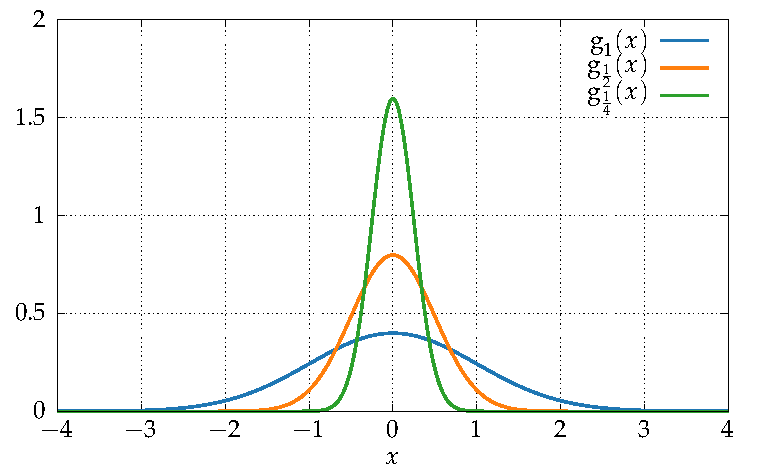
\includegraphics{gp_gauss.pdf}
  \caption{Curve of the Gaussian kernel defined in \cref{def:gauss} for several widths.}
  \label{fig:gauss}
\end{figure}
\begin{example}
  The function $f$ defined for $x\in\R$ by
  \begin{equation}
    f(x)=\frac{1}{x^2+2}\,,
  \end{equation}
  is not a Schwartz function, although it is infinitely differentiable. Indeed,
  \begin{equation}
    \lim_{x\to+\infty} x^2\,f(x)=1\,,
  \end{equation}
  which does not satisfy~\cref{def:schwartz-fn}. It is, however, a function of moderate
  growth.
\end{example}
\begin{example}
  The function $f$ defined for $x\in\R$ by
  \begin{equation}
    f(x)=e^{-|x|}\,,
  \end{equation}
  is not a Schwartz function, although it is a rapidly decaying function. Indeed,
  \begin{equation}
    f'(x)=-\sign(x)\,e^{-|x|}\,,
  \end{equation}
  is discontinuous at $0$, and therefore $f$ does not admit a second derivative.
\end{example}
\begin{example}
  All polynomials are functions of moderate growth, but the exponential function is not a
  function of moderate growth.
\end{example}
We also generalise the dot product introduced in~\cref{def:func-dot}
\begin{definition}
  Let $f$ be a Schwartz function on $\R$, and $g$ be an integrable moderately growing
  function on $\R$. We define the \emph{dot product} $\braket{f,g}$ of $f$ and $g$ with
  the following integral
  \begin{equation}
    \braket{f,g}=\intr{x}f(x)g(x)^*\,.
  \end{equation}
  Additionally, the norm $\|f\|$ of a Schwartz function $f$ is defined by
  \begin{equation}
    \|f\|^2=\braket{f,f}=\intr{x}|f(x)|^2
  \end{equation}
\end{definition}
It is important to note that the norm of a moderately growing function and the dot product
of two moderately growing functions are generally not well-defined, as the associated
integrals might not converge. Schwartz functions have the following simple integration by
parts formula.
\begin{proposition}
  Let $f$ be a Schwartz function on $\R$, and let $g$ be a continuously differentiable
  function of moderate growth. Then we have the integration by parts formula
  \begin{equation}
    \intr{x}f'(x)g(x)=-\intr{x}f(x)g'(x)\,.
  \end{equation}
  Or, equivalently, $\braket{f',g}=-\braket{f,g'}$.
\end{proposition}
\begin{proof}
  Let $A$ be a positive real number, we have
  \begin{equation}
    \int_{-A}^A\diff x\,f'(x)g(x)=[f(x)g(x)]_{-A}^A-\int_{-A}^A\diff x\,f(x)g'(x)\,.
  \end{equation}
  Using \cref{prop:rapid-times-moderate}, $fg$ is a rapidly decaying function so
  \begin{equation}
    \lim_{A\to+\infty}[f(x)g(x)]_{-A}^A=0\,.
  \end{equation}
  Taking the same limit in the two integrals above proves the proposition.
\end{proof}
We are now ready to define the Fourier transform:
\begin{definition}
  Let $f$ be an integrable function on $\R$, the function $\hat{f}$ defined on $\R$ by
  \begin{equation}
    \hat{f}(\omega)=\int_{-\infty}^{+\infty}\diff x\,f(x)\,e^{-2\pi i\omega x}\,,
  \end{equation}
  is called the \emph{Fourier transform} of $f$. We additionally note $\mathcal{F}$ the
  operator that associates $f$ to its Fourier transform $\mathcal{F}f=\hat{f}$.
\end{definition}
Clearly, all Schwartz functions are integrable and therefore have a well-defined
Fourier transform. However, one can question the properties of the Fourier transform,
and whether the duality conjectured in~\cref{eq:ft-conjecture} holds. Through the example
below, which is a classical result in Fourier analysis, we can see that rapidly decaying
functions do not necessarily have a rapidly decaying Fourier transform.
\begin{figure}[t]
  \centering
  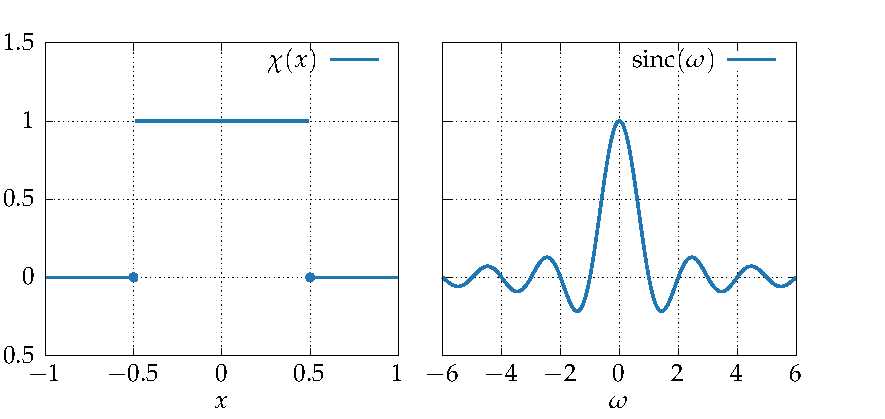
\includegraphics{gp_sinc-ft.pdf}
  \caption{This figure illustrates~\cref{ex:sinc-ft}. The indicator function of the interval $(-\frac{1}{2},\frac{1}{2})$ defined in~\cref{eq:int-indicator} is represented in the left pane. The right pane represents its Fourier transform, the sine cardinal function.}
  \label{fig:sinc-ft}
\end{figure}
\begin{example}
  \label{ex:sinc-ft}
  Let $\chi$ the function on $\R$ defined by
  \begin{equation}
    \chi(x)=
    \begin{cases}
      1&\text{if}~-\frac{1}{2}<x<\frac{1}{2}\\
      0&\text{else}
    \end{cases}\,,
    \label{eq:int-indicator}
  \end{equation}
  for all $x\in\R$. $\chi$ is a rapidly decaying function, but it is not a Schwartz
  function as it has discontinuities in $-1$ and $1$. Its Fourier transform is given by
  \begin{equation}
    \hat{\chi}(\omega)=\int_{-\frac12}^{\frac12}\diff x\,e^{-2\pi i\omega x}=
    -\frac{1}{2\pi i\omega}(e^{-\pi i\omega}-e^{\pi i\omega})=\frac{\sin(\pi\omega)}{\pi\omega}\,.
  \end{equation}
  The function $\hat{\chi}(\omega)$ is called the \emph{sine cardinal function} and
  is generally noted $\sinc$:
  \begin{equation}
    \sinc(x)=\frac{\sin(\pi x)}{\pi x}\,.
  \end{equation}
  Although this function has an apparent singularity at $x=0$, $\sin(\pi x)\simeq \pi x$
  for $x\to0$, therefore $\sinc$ can be continued to the finite value $\sinc(0)=1$.
  $\chi$ and its Fourier transform are illustrated in~\cref{fig:sinc-ft}.
  We can observe that although $\chi$ is rapidly decaying, its Fourier transform is not.
  This is related to the lack of smoothness of $\chi$. As we will see below, this is not
  an issue with Schwartz functions.
\end{example}
As in the case of Fourier coefficients (\cref{prop:fourier-coef-trans}), the Fourier
transform admits some useful transformation identities. We start by defining the
conjugation and scaling operators.
\begin{definition}
  For any function $f$ on $\R$, we define the \emph{conjugation operator} $\mathcal{C}$
  which associates to $f$ its complex conjugate $\mathcal{C}f=f^*$.
\end{definition}
\begin{definition}
  For any function $f$ on $\R$, and any positive real number $\delta$, we define the
  \emph{scaling operator} $\mathcal{S}_{\delta}$ which associates to $f$ the function
  defined by $\mathcal{S}_{\delta}f(x)=f(\delta x)$, for all $x\in\R$.
\end{definition}
\begin{proposition}
  The conjugation, reflection, translation, and scaling of a Schwartz function are still
  Schwartz functions.
\end{proposition}
Then we have the following transformation rules.
\begin{proposition}
  \label{prop:ft-trans}
  Let $f$ be a Schwartz function on $\R$, the following properties hold
  \begin{enumerate}
    \item \emph{Conjugation}: $\mathcal{F}(f^*)(\omega)=[\hat{f}(-\omega)]^*$, or
      $\mathcal{F}\mathcal{C}=\mathcal{C}\mathcal{R}\mathcal{F}$.
    \item \emph{Reflection}: $\mathcal{F}(\tilde{f})(\omega)=\hat{f}(-\omega)$, or
      $\mathcal{F}\mathcal{R}=\mathcal{R}\mathcal{F}$.
    \item \emph{Translation}: For $a\in\R$, $(\mathcal{F}\mathcal{T}_{a})f(\omega)
      =e^{-2\pi i\omega a}\hat{f}(\omega)$, or
      $\mathcal{F}\mathcal{T}_{a}=\ew(-a)\mathcal{F}$.
    \item \emph{Scaling}: For $\delta\in\R$ with $\delta>0$,
      $(\mathcal{F}\mathcal{S}_{\delta})f(\omega)=\delta^{-1}\hat{f}(\delta^{-1}\omega)$,
      or
      $\mathcal{F}\mathcal{S}_{\delta}=\delta^{-1}\mathcal{S}_{\delta^{-1}}\mathcal{F}$.
    \item \emph{Differentiation in space:} For $\alpha$ a non-negative integer,
      $\mathcal{F}(f^{(\alpha )})=(2\pi i\omega)^{\alpha}\hat{f}(\omega)$.
    \item \emph{Differentiation in frequency:} For $\alpha$ a non-negative integer,
      $\hat{f}$ is $\alpha$ times differentiable. Let $g$ the function defined for
      $x\in\R$ by $g(x)=(-2\pi ix)^\alpha f(x)$, then $\hat{g}=\hat{f}^{(\alpha)}$.
  \end{enumerate}
\end{proposition}
\begin{proof}
  The proof of this proposition is part of the exercises of this chapter.
\end{proof}
A first important property of Schwartz function is that their decay and smoothness
properties are preserved by the Fourier transform:
\begin{theorem}
  If $f$ is a Schwartz function, then its Fourier transform $\hat{f}$ is also a Schwartz
  function.
\end{theorem}
\begin{proof}
  Let us first observe that the Fourier transform of a Schwartz function always goes to
  zero at infinity, which is a variant of the Riemann-Lebesgue lemma for Schwartz
  functions. Using \cref{prop:ft-trans}, we know that for $\omega\neq 0$,
  \begin{equation}
    \hat{f}(\omega)=\frac{1}{2\pi i\omega}\mathcal{F}(f')\,.\label{eq:ft-ip}
  \end{equation}
  Since $f'$ is a Schwartz function, its Fourier transform is bounded by
  \begin{equation}
    |\mathcal{F}(f')|=\left|\intr{x}f'(x)\,e^{-2\pi i \omega x}\right|\leq
    \intr{x}|f'(x)|\,,
  \end{equation}
  therefore taking $|\omega|\to+\infty$ in~\cref{eq:ft-ip}, we get
  \begin{equation}
    \lim_{|\omega|\to+\infty}\hat{f}(\omega)=0
  \end{equation}
  Now, let $\alpha$ and $\beta$ be two non-negative integers. Then, using
  \cref{prop:ft-trans}, for all $\omega\in\R$,
  \begin{equation}
    \omega^\beta\hat{f}^{(\alpha)}(\omega)=\frac{1}{(2\pi i)^{\beta}}\mathcal{F}(f^{(\alpha+\beta)})(\omega)\,.
  \end{equation}
  Since $f^{(\alpha+\beta)}$ is a Schwartz function (\cref{prop:schwartz-comb}), then as
  discussed above its Fourier transform goes to zero at infinity, and therefore
  \begin{equation}
    \lim_{|\omega|\to+\infty}\omega^\beta\hat{f}^{(\alpha)}(\omega)=0\,,
  \end{equation}
  which proves that $\hat{f}$ is a Schwartz function.
\end{proof}
Another important property is the Fourier transform of Gaussian kernels.
\begin{theorem}[Gaussian uncertainty principle]
  \label{thm:gauss-uncertainty}
  The Fourier transform of a Gaussian kernel of width $\sigma$ is, up to proportionality
  factor, a Gaussian kernel of width $\hat{\sigma}=\frac{1}{2\pi\sigma}$:
  \begin{equation}
    \hat{\gauss}_{\sigma}(\omega)=
    \frac{1}{\sigma\sqrt{2\pi}}\gauss_{\hat{\sigma}}(\omega)
    =e^{-2\pi^2\sigma^2\omega^2}\,.
  \end{equation}
  In particular,
  \begin{equation}
    \sigma\hat{\sigma}=\frac{1}{2\pi}\,.\label{eq:gauss-uncertainty}
  \end{equation}
\end{theorem}
\begin{proof}
  The proof of this proposition is part of the exercises of this chapter.
\end{proof}
The theorem above is called the ``uncertainty principle'' in reference to the original work
of physicist Werner Heisenberg in quantum mechanics, where this relationship was first observed.
However, it is important to note that it has a wide range of implications and interpretations
beyond quantum mechanics. The general interpretation is that if the resolution of an object in space is dictated by a Gaussian distribution of a given width, then the associated distribution in frequency has the inverse width. A direct consequence is that it is impossible to achieve arbitrarily high resolution both in space and frequency simultaneously, hence the ``uncertainty''.
%-----------------------------------------------------------------------------------------
\subsection{Convolution product}
A key operation in Fourier analysis is the \emph{convolution product}. When convoluting a
function $f$ by another function $g$, one averages from a given point $x$ the values of $f$
according to the weights given by $g$:
\begin{definition}
  Let $f$ and $g$ be two functions on $\R$ such that the integral
  \begin{equation}
    (f\ast g)(x)=\intr{y}f(x-y)g(y)\label{eq:conv-def}
  \end{equation}
  is well-defined and finite for all $x\in\R$. The function $f\ast g$ defined on $\R$ by
  the relation above is called the \emph{convolution product} of $f$ and $g$.
  The convolution product can also be written as the dot product
  \begin{equation}
    (f\ast g)(x)=\braket{\mathcal{R}\mathcal{T}_xf,g^*}\,.
  \end{equation}
\end{definition}
Convolution products are bilinear and commutative:
\begin{proposition}
  Let $f$, $g$ and $h$ three functions on $\R$ such that $f\ast g$ and $f\ast h$ are
  well-defined. Then,
  \begin{equation}
    f\ast g=g\ast f\,,
  \end{equation}
  and for all pairs of complex numbers $a$, $b$,
  \begin{equation}
    f\ast (ag+bh)=a(f\ast g) + b(f\ast h)\,.
  \end{equation}
\end{proposition}
\begin{proof}
  The commutation property is obtained by using the change of variable
  $z=x-y$ in the definition \cref{eq:conv-def}. The second formula is a trivial consequence
  of the integral linearity.
\end{proof}
Convolution products have crucial regularisation properties. Roughly speaking, a product
$f\ast g$ will have the smoothness properties of the smoothest function between $f$
and $g$. In particular, convoluting by a Schwartz function leads to a Schwartz function:
\begin{theorem}
  Let $f$ be a Schwartz function on $\R$ and $g$ be an integrable moderately growing
  function on $\R$. The convolution product $f\ast g$ is a Schwartz function and for all
  non-negative integers $\alpha$,
  \begin{equation}
    (f\ast g)^{(\alpha)}=f^{(\alpha)}\ast g\,.
  \end{equation}
\end{theorem}
\begin{proof}
  We will largely admit this result. However, it is not too difficult to see that it is
  correct if one can freely exchange the integral in~\cref{eq:conv-def} with derivatives
  and limits in $x$. For example
  \begin{equation}
    (f\ast g)'(x)=\frac{\diff}{\diff x}\intr{y}f(x-y)g(y)=
    =\intr{y}f'(x-y)g(y)\,,
  \end{equation}
  and for a non-negative integer $\alpha$,
  \begin{equation}
    \lim_{|x|\to+\infty}x^{\alpha}(f\ast g)(x)=
    \intr{y}\left[\lim_{|x|\to+\infty}x^{\alpha}f(x-y)\right]g(y)=0\,.
  \end{equation}
  One can show that the exchange of limit and integral is a consequence of the integrand
  being a rapidly decaying function (\cref{prop:rapid-times-moderate}), which is the part
  we are admitting here.
\end{proof}
\begin{theorem}
  \label{thm:gaussian-unit}
  Let $f$ be a Schwartz function on $\R$, then $f\ast \gauss_{\sigma}$ converges uniformly
  to $f$ for $\sigma\to 0$.
\end{theorem}
\begin{proof}
  We will largely admit this result, and give a heuristic proof instead. For $y\neq 0$, by definition
  \begin{equation}
    \lim_{\sigma\to 0}\gauss_{\sigma}(y)=0
  \end{equation}
  exponentially fast. Let $\eta$ be a small positive real number, we write
  \begin{equation}
    (f\ast \gauss_{\sigma})(x)=\intr{y}f(x-y)\gauss_{\sigma}(y)\,.
  \end{equation}
  Changing the variable with $y=\sigma z$, we obtain
  \begin{equation}
    (f\ast \gauss_{\sigma})(x)=\intr{y}f(x-\sigma z)\gauss_{1}(y)\,.
  \end{equation}
  Assuming we can exchange limit and integral, and using the fact that $f$ is continuous,
  \begin{equation}
    \lim_{\sigma\to 0}(f\ast \gauss_{\sigma})(x)=f(x)\intr{y}\gauss_{1}(y)=f(x)\,.
  \end{equation}
\end{proof}
\begin{corollary}
  Let $f$ be a Schwartz function on $\R$, we have the following limit
  \begin{equation}
    \lim_{\sigma\to0}\braket{f,\gauss_{\sigma}}=f(0)\,.
  \end{equation}
\end{corollary}
\begin{proof}
  One first observes that
  \begin{equation}
    (\tilde{f}\ast g)(x)=\intr{y}f(y-x)\gauss_{\sigma}(y)\,,
  \end{equation}
  therefore
  \begin{equation}
    \braket{f,\gauss_{\sigma}}=(\tilde{f}\ast g)(0)\,,
  \end{equation}
  which proves the corollary using~\cref{thm:gaussian-unit}.
\end{proof}
%-----------------------------------------------------------------------------------------
\subsection{Inverse Fourier transform}
\begin{theorem}[Multiplication formula]
  Let $f$ and $g$ be two Schwartz functions on $\R$, then
  \begin{equation}
    \intr{x}\hat{f}(x)g(x)=\intr{x}f(x)\hat{g}(x)\,.
  \end{equation}
\end{theorem}
\begin{corollary}
  Let $f$ and $g$ be two Schwartz functions on $\R$, then
\end{corollary}
\begin{theorem}[Fourier inversion]
  Let $f$ be a Schwartz function on $\R$, then for all $x\in\R$,
  \begin{equation}
    f(x)=\intr{\omega}\hat{f}(\omega)\,e^{2\pi i\omega x}\,.
  \end{equation}
  In other words, the Fourier transform is an invertible operation, and
  $\mathcal{F}^{-1}=\mathcal{R}\mathcal{F}$.
\end{theorem}
\begin{corollary}
  We have the following identities
  \begin{equation}
    \mathcal{F}^2=\mathcal{R}\qquad\text{and}\qquad\mathcal{F}^4=1\,,
  \end{equation}
  \ie two successive Fourier transforms are equivalent to a reflection, and four
  successive Fourier transforms are equivalent to no transformation.
\end{corollary}
%-----------------------------------------------------------------------------------------
\subsection{Plancherel formula}
\begin{theorem}[Convolution theorem]
  Let $f$ and $g$ be two Schwartz functions on $\R$, then
  \begin{equation}
    \mathcal{F}(f\ast g)=\hat{f}\,\hat{g}\qquad\text{and}\qquad
    \mathcal{F}(fg)=\hat{f}\ast\hat{g}\,.
  \end{equation}
\end{theorem}
\begin{theorem}[Plancherel]
  Let $f$ be a Schwartz function on $\R$, then $\|f\|=\|\hat{f}\|$.
\end{theorem}
%%%%%%%%%%%%%%%%%%%%%%%%%%%%%%%%%%%%%%%%%%%%%%%%%%%%%%%%%%%%%%%%%%%%%%%%%%%%%%%%%%%%%%%%%%
\section{Generalised functions -- \textit{There be dragons}}
%%%%%%%%%%%%%%%%%%%%%%%%%%%%%%%%%%%%%%%%%%%%%%%%%%%%%%%%%%%%%%%%%%%%%%%%%%%%%%%%%%%%%%%%%%
\section{Back to Fourier series}
%%%%%%%%%%%%%%%%%%%%%%%%%%%%%%%%%%%%%%%%%%%%%%%%%%%%%%%%%%%%%%%%%%%%%%%%%%%%%%%%%%%%%%%%%%
\section{Inversion of differential operators}